\documentclass[11pt]{article}

% Change "review" to "final" to generate the final (sometimes called camera-ready) version.
% Change to "preprint" to generate a non-anonymous version with page numbers.
\usepackage[review]{acl}

% Standard package includes
\usepackage{times}
\usepackage{latexsym}
\usepackage[T1]{fontenc}
\usepackage[utf8]{inputenc}
\usepackage{microtype}
\usepackage{inconsolata}
\usepackage{graphicx}
\usepackage{booktabs}
\usepackage{amsmath}
\usepackage{amssymb}

\graphicspath{{../../figures/final/}{../figures/final/}{figures/final/}{./}}

\newcommand{\acc}{Accuracy@1}
\newcommand{\rone}{Recall@1}

\title{When Does the LLM Disambiguation Stage Actually Help?\\
A Decomposition of Retriever--LLM Interaction in Biomedical Entity Linking}

\author{First Author \\
  Affiliation / Address line 1 \\
  Affiliation / Address line 2 \\
  \texttt{email@domain} \\\And
  Second Author \\
  Affiliation / Address line 1 \\
  Affiliation / Address line 2 \\
  \texttt{email@domain} \\\And
  Third Author \\
  Affiliation / Address line 1 \\
  Affiliation / Address line 2 \\
  \texttt{email@domain} \\}

\begin{document}
\maketitle

\begin{abstract}
Large language models are routinely bolted onto biomedical entity-linking (EL)
pipelines as a final disambiguation stage, and recent work reports large gains from
doing so. We do not propose a new method: we ask \emph{how much}, \emph{when}, and
\emph{why} this stage helps. Using a reproduced neuro-symbolic pipeline as a
measuring instrument, we run one fixed open 4B disambiguator behind fourteen
retriever configurations spanning five corpora (BC5CDR, BioRED, NCBI-Disease,
NLM-Chem, MedMentions) and four retrievers, including two public systems we did not
build. Four results follow. (i) The stage's contribution is set by the retriever,
not by the model: it ranges from $+0.6$ to $+10.1$ \acc{} points with the same model
and prompt, and \emph{within} a corpus a stronger retriever reliably means a smaller
gain (12/14 ordered pairs; dataset-demeaned $\rho=-0.72$, $p=0.004$). Degrading one
retriever's ranking in graded steps on a fixed candidate pool makes this causal: the
stage absorbs $89\%$ of the accuracy the retriever gives up, linearly
($r=-1.0000$). (ii) The
zero-shot model's intervention rate is well calibrated but its intervention
precision is not: precision collapses in a \emph{mid-confidence} band where the
retriever is already right, making the stage net-harmful there; this survives three
prompt ablations, including one that states the retriever's margin as a number and
instructs the model to defer on large margins. (iii) LoRA fine-tuning does not improve the model where
disambiguation is hard---precision on the truly-uncertain band is unchanged---but
installs a confidence-dependent \emph{restraint} whose reliability benefit is bound
to the training distribution: over three seeds, on held-out corpora it raises
intervention precision from $69\%$ to $91\%$ on concepts seen in fine-tuning while on
unseen ones precision does not improve at all ($72\% \to 70\%$). (iv) A $109$M-parameter
cross-encoder on the identical candidate lists beats the $4$B LLM in-domain
($+2.1$ points, CI excluding zero) and loses to it on the corpus furthest from its
training data, so what the generative stage buys is transfer rather than
disambiguation as such --- and it reproduces the same net-harmful band once its
interventions stop tracking retriever confidence, which places that failure outside
language models entirely. We release all prediction dumps and analysis code.
\end{abstract}

\section{Introduction}

Biomedical entity linking maps a mention in text to a concept in a knowledge base
such as MeSH or UMLS \citep{bodenreider-2004-umls}. Most systems are two-stage: a
retriever proposes candidate concepts, and a disambiguation stage selects among them.
Large language models (LLMs) are now the default choice for the second stage.
\citet{ye-mitchell-2025-llm} report a new state of the art---up to $+16$ points---from
a training-free LLM disambiguator placed on top of an existing retriever, and
\citet{lin-etal-2025-guiding} obtain competitive results by constraining the decoder.
The field treats this stage as a semantic reasoner that supplies what the retriever
cannot.

A single accuracy number cannot support that reading. It hides where the stage helps,
where it hurts, and what fine-tuning changes about it. It also hides how much of the
reported gain is a property of the LLM at all, as opposed to a property of the
retriever it was placed behind: the same disambiguator behind a weak retriever has far
more to fix than behind a strong one, so ``$+16$ points'' is a statement about a pair
of components, not about one of them.

We therefore reframe the problem from ``build a better system'' to ``characterise a
stage the field has not yet characterised''. We reproduce the neuro-symbolic
BioLinkerAI pipeline \citep{sakor-etal-2024-biolinkerai} and use it as an
instrument: we hold the disambiguator, the prompt and the mention set fixed and vary
only the retriever, across fourteen configurations and five corpora. Our
contributions are:

\begin{enumerate}\itemsep1pt
\item \textbf{The frame} (\S\ref{sec:frame}). The stage's marginal value is a
decreasing function of retriever strength. \citet{ye-mitchell-2025-llm} note this
qualitatively over two base models; we measure it over fourteen configurations, show
it is identified \emph{within} a corpus and not across corpora, and then manipulate
it directly: degrading one retriever's ranking in graded steps on a fixed candidate
pool, the stage absorbs $89\%$ of the accuracy lost, linearly ($r=-1.0000$).
\item \textbf{A mid-confidence danger zone} (\S\ref{sec:f1}). The intervention
\emph{rate} falls with retriever confidence but the intervention \emph{precision}
collapses in a middle band, where the model over-rides a mostly-correct retriever. It
survives three prompt ablations, a surface-similarity control and an external
retriever's confidence signal.
\item \textbf{Deference, not competence} (\S\ref{sec:f2}). Fine-tuning leaves
precision flat on the cases the retriever cannot solve and instead learns \emph{when}
not to act; the reliability it buys is realised almost entirely on concepts present
in the fine-tuning data.
\end{enumerate}

\section{Related Work}

\paragraph{Biomedical EL and the LLM stage.}
BioLinkerAI \citep{sakor-etal-2024-biolinkerai} is a neuro-symbolic pipeline
(linguistic rules, candidate generation, domain rules, LLM disambiguation) that we
reproduce as our instrument. \citet{ye-mitchell-2025-llm} isolate the LLM as a
disambiguator on top of SapBERT and ArboEL and observe qualitatively, over two fixed
base models, that its value depends on the base model's strength; we make that
relation quantitative, identify it within corpora, and extend it to fine-tuning.
\citet{lin-etal-2025-guiding} guide the LLM with restrictive and contrastive decoding;
their own ablations show the LLM machinery adds $\leq 0.3$ points on BC5CDR, which is
indirect support for our frame. The current state of the art is a trained generative
model, ANGEL \citep{kim-etal-2025-angel}; it has no separable retriever stage and is
orthogonal to our analysis. Our retrievers are a lexical/BM25 baseline, SapBERT
\citep{liu-etal-2021-self}, BioSyn \citep{sung-etal-2020-biomedical} and the
reproduced rule pipeline.

\paragraph{Selective prediction and confidence gating.}
Abstaining on low-confidence inputs is long-standing in selective classification
\citep{geifman-elyaniv-2017-selectivenet} and, for LLM pipelines, in cascaded routing
\citep{chen-etal-2023-frugalgpt}. Our setting inverts the polarity: we abstain from
\emph{intervening} rather than from predicting, and the confidence signal belongs to
the upstream retriever, not to the model being gated. \citet{doku-2026-confidence}
call the failure mode we observe an ``inversion zone''.

\paragraph{Memorisation under fine-tuning.}
That fine-tuning trades cross-domain generalisation for in-domain performance is known
for EL retrievers \citep{logeswaran-etal-2019-zero}. Our contribution is the
mechanism for the LLM disambiguation stage, with a zero-shot control on the same
mentions: what transfers is not accuracy but restraint, and only in-distribution.

\section{Experimental Setup}\label{sec:setup}

\paragraph{Pipeline.}
We use our reproduction of BioLinkerAI: candidate generation (P2), rule-based
re-ranking (P3), and LLM disambiguation (P4). P2 matches the mention against a MeSH
index (descriptors and supplementary concepts) enriched with synonyms harvested from
UMLS, Wikidata and DBpedia, after an abbreviation-expansion pass; P3 re-ranks with
hand-written domain rules and emits a top-10 candidate list with scores. Throughout,
P3 denotes the retriever's final top-1 and P4 the pipeline's output; the stage's
effect is $\Delta = \text{P4}-\text{P3}$ in \acc{} points. Mentions are
gold-annotated: we evaluate linking, not detection. Where a run is labelled with a
standalone retriever (BM25, SapBERT, BioSyn), P2 and P3 are replaced wholesale by
that system's ranked list and scores, and only P4 is ours.

\paragraph{Disambiguator.}
Qwen3-4B \citep{yang-etal-2025-qwen3} served with vLLM
\citep{kwon-etal-2023-efficient}, temperature $0$, with a fixed prompt and decoding
constrained to an enumeration over the candidate list, so the stage can only select
among P3's candidates and never invents an identifier. It runs in two variants:
zero-shot, and LoRA \citep{hu-etal-2022-lora} supervised fine-tuning on the BC5CDR
training split (chat format, completion-only loss, at most five examples per
mention--concept pair, no in-context examples). All runs share the same prompt, the
same decoding settings and the same top-10 candidate lists, so every difference we
report is attributable to the retriever or to the fine-tuning, never to the
interface.

\paragraph{Corpora and retrievers.}
BC5CDR \citep{li-etal-2016-biocreative}, BioRED \citep{luo-etal-2022-biored},
NCBI-Disease \citep{dogan-etal-2014-ncbi} and NLM-Chem
\citep{islamaj-etal-2021-nlmchem} are linked against MeSH; MedMentions
\citep{mohan-li-2019-medmentions} against the full UMLS. Following the BioLinkerAI
evaluation protocol we keep duplicate mention strings, which inflates absolute
accuracies relative to de-duplicated protocols \citep{tutubalina-etal-2020-fair}; all
comparisons here are between systems on the identical mention set, so this does not
affect any $\Delta$. Table~\ref{tab:runs} lists the fourteen retriever
configurations. BM25 and BioSyn are standalone public systems we did not build; for
those runs the LLM stage sees only that system's candidates and scores. Two entries in
that table need a word. On NCBI-Disease dense retrieval is \emph{worse} than lexical
matching (\rone{} $60.7$ vs.\ $71.3$): the corpus is dominated by short disease
abbreviations and modifier phrases whose surface form is highly diagnostic, which
SapBERT's embedding space blurs. And the two MedMentions runs cover $4{,}823$ and
$5{,}000$ mentions; where they are compared directly (\S\ref{sec:frame}) we restrict to
the $4{,}823$ they share.

\paragraph{A reproduction, not a replication.}
Our pipeline follows BioLinkerAI's architecture but does not reach its reported
accuracy: on BC5CDR we obtain $83.7$ against the $93.3$ reported there with GPT-4, and
on MedMentions $59.6$ against $81.3$. Neither the code nor the prompts were released
and the reported system uses a closed-source disambiguator, so we cannot attribute the
gap; it may lie in candidate generation, in the knowledge-base snapshot, in the
disambiguator, or in evaluation details. We therefore do not present this pipeline as
a replication or as a competitive system, and we make no cross-paper accuracy claims.
It is used only as a controlled instrument: every comparison we report holds the
mention set, the candidate lists, the prompt and the decoder fixed and varies one
component, so a constant offset in absolute accuracy does not affect any $\Delta$. The
two standalone public retrievers (BM25 and BioSyn) additionally check that the effects
are not artefacts of our own candidate generation and scoring.

\paragraph{Confirmatory vs.\ descriptive analyses.}
The band-level breakdowns are descriptive: they slice five confidence bands across five
corpora and two model variants, and we do not correct their intervals for
multiplicity. Three analyses are confirmatory and carry the paper's claims: the
within-corpus relation between retriever strength and the stage's gain
(\S\ref{sec:frame}), the seen-versus-unseen precision contrast (\S\ref{sec:f2}), and
the gated-versus-full comparison (\S\ref{sec:f1}). Each is a single pre-specified
test.

\paragraph{Metrics.}
\emph{Candidate \rone{}} is the retriever's top-1 accuracy and our measure of
retriever strength; \emph{\rone{}@10} (the gold concept appearing anywhere in the
candidate list) bounds what the stage could possibly recover. We report the
\emph{intervention rate} (share of mentions whose top-1 the LLM changes), the
\emph{intervention precision} $\mathrm{fixes}/(\mathrm{fixes}+\mathrm{breaks})$, and
$\Delta$. Retriever confidence is the top1$-$top2 score gap after P3. Score scales
differ across retrievers, so confidence is always binned \emph{within} a run, either
into fixed gap bands or by percentile. Confidence intervals are 95\% document-level
bootstrap \citep{efron-1979-bootstrap} resampling PMIDs, since mentions inside one
abstract are correlated.

\begin{table}[t]
\centering\footnotesize
\setlength{\tabcolsep}{2.6pt}
\begin{tabular}{llrrrrr}
\toprule
Corpus & Retriever & \multicolumn{1}{c}{$n$} & R@1 & R@10 & P4 & $\Delta$ \\
\midrule
BC5CDR & BM25 & 9{,}391 & 73.4 & 79.1 & 75.4 & +2.0 \\
 & SapBERT & 9{,}661 & 75.9 & 87.3 & 80.6 & +4.6 \\
 & pipeline & 9{,}661 & 82.7 & 91.6 & 83.7 & +0.9 \\
 & BioSyn & 9{,}661 & 84.8 & 90.5 & 85.4 & +0.6 \\
\addlinespace[2pt]
BioRED & SapBERT & 1{,}661 & 70.8 & 86.5 & 77.9 & +7.1 \\
 & lexical & 1{,}661 & 74.2 & 88.1 & 82.1 & +7.9 \\
 & pipeline & 1{,}661 & 79.5 & 93.6 & 83.6 & +4.0 \\
\addlinespace[2pt]
NCBI & SapBERT & 863 & 60.7 & 78.6 & 64.2 & +3.5 \\
 & pipeline & 863 & 70.1 & 90.0 & 72.5 & +2.4 \\
 & lexical & 863 & 71.3 & 84.4 & 72.8 & +1.5 \\
\addlinespace[2pt]
NLM-Chem & lexical & 1{,}500 & 65.9 & 81.0 & 76.0 & +10.1 \\
 & dense & 1{,}500 & 72.3 & 86.9 & 78.0 & +5.7 \\
\addlinespace[2pt]
MedMent. & lexical & 4{,}823 & 49.6 & 71.4 & 58.4 & +8.9 \\
 & SapBERT & 5{,}000 & 55.3 & 77.3 & 59.6 & +4.3 \\
\bottomrule
\end{tabular}
\caption{The fourteen retriever configurations, ordered by retriever strength within
each corpus. All use the same zero-shot Qwen3-4B disambiguator and the same prompt.
R@1 is the retriever's top-1 accuracy, R@10 the share of mentions whose gold concept
appears anywhere in the candidate list (the ceiling for the LLM stage), P4 the final
\acc{}, and $\Delta = \text{P4}-\text{R@1}$.}
\label{tab:runs}
\end{table}

\paragraph{Reproducibility.}
Every number in this paper is recomputed from per-mention prediction dumps that record,
for each mention, the retriever's top-1 and its score gap, the pipeline's output,
whether either was correct, whether the gold concept appeared in the candidate list
and at what rank. The dumps, the analysis scripts and the figure scripts are released;
no model inference is needed to reproduce any table or figure here.

\section{The Frame: the Retriever Sets the LLM's Value}\label{sec:frame}

\begin{figure*}[t]
\centering
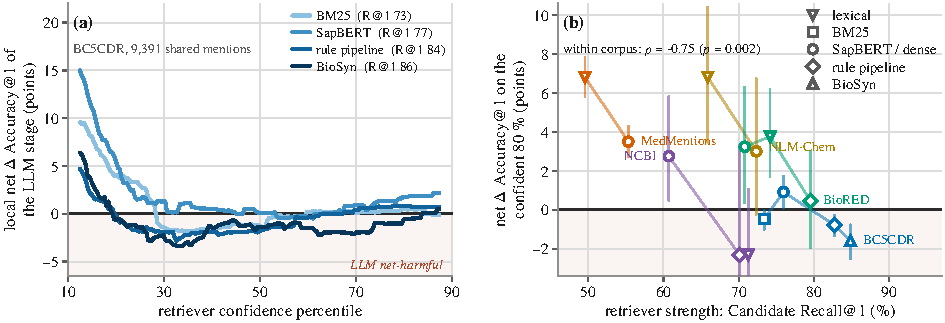
\includegraphics[width=\textwidth]{fig1_value.pdf}
\caption{\textbf{Where along the retriever's own confidence the LLM stage pays off.}
\textbf{(a)} Local net $\Delta$ \acc{} in a sliding window covering 25\% of each run,
over the percentile of that run's top1$-$top2 score gap; BC5CDR, four retrievers,
restricted to the 9{,}391 mentions all four cover. Every profile is strongly positive
where the retriever is unsure, and the whole curve moves down as the retriever
strengthens: behind BioSyn and the rule pipeline it crosses into the net-harmful
region in the \emph{middle} of the confidence range. \textbf{(b)} All fourteen runs:
net $\Delta$ \acc{} on the 80\% of mentions the retriever is most confident about,
with document-level bootstrap 95\% CIs. Thin lines join runs on the same corpus, which
is where the effect is identified; pooled across corpora the relation is confounded by
how hard each corpus is.}
\label{fig:value}
\end{figure*}

The same model with the same prompt contributes between $+0.6$ and $+10.1$ points
depending only on what precedes it (Table~\ref{tab:runs}): a seventeen-fold range with the model, the prompt and the
candidate-list size held constant.
The interesting question is whether that spread is systematic.

Pooled across all fourteen runs it is not clearly so: $\Delta$ correlates with
Candidate \rone{} at $\rho=-0.50$ ($p=0.069$), because corpus difficulty confounds
the comparison. The effect is identified \emph{within} a corpus, where the mention
set and the knowledge base are held fixed: there, 12 of the 14 ordered pairs put the
smaller gain behind the stronger retriever (sign test $p=0.013$), and after removing
corpus means the relation is $\rho=-0.72$ ($p=0.004$; OLS slope $-0.32$ gain points
per point of \rone{}, $r=-0.76$). The two exceptions are cases where the
``stronger'' retriever also changed the candidate pool substantially. De-duplicating
the test sets keeps the correlation ($\rho=-0.67$, $p=0.009$) but not the sign test
($10/14$, $p=0.18$), so we state the relation as graded rather than as a rule that
holds pair by pair --- and in \S\ref{sec:dose} we stop inferring it and manipulate
it.

A direct consequence is that the two components are partial \emph{substitutes}: on
the same MedMentions mentions, moving from lexical to SapBERT retrieval buys $+7.3$
points of \rone{} but only $+2.7$ points of final accuracy, and on BC5CDR replacing
SapBERT with BioSyn buys $+8.9$ and $+4.9$. Investment in the retriever has
diminishing final returns because the LLM stage was masking the retriever's
weakness. \S\ref{sec:dose} measures that substitution directly.

Figure~\ref{fig:value}a shows where in the pipeline this happens. With the retriever
varied on a fixed BC5CDR mention set, every configuration's value profile is strongly
positive at low retriever confidence and flat-to-negative at high confidence; what
changes with retriever strength is the \emph{level} of the whole curve. Summarising
each run by its $\Delta$ on the confident 80\% of its mentions (Figure~\ref{fig:value}b)
gives the same within-corpus relation, more sharply: $\rho=-0.75$ ($p=0.002$;
$r=-0.85$, $p=0.0001$). Behind the strongest retrievers this quantity is negative --- the
stage is a net cost on everything except the mentions the retriever is least sure
about.

\begin{figure*}[t]
\centering
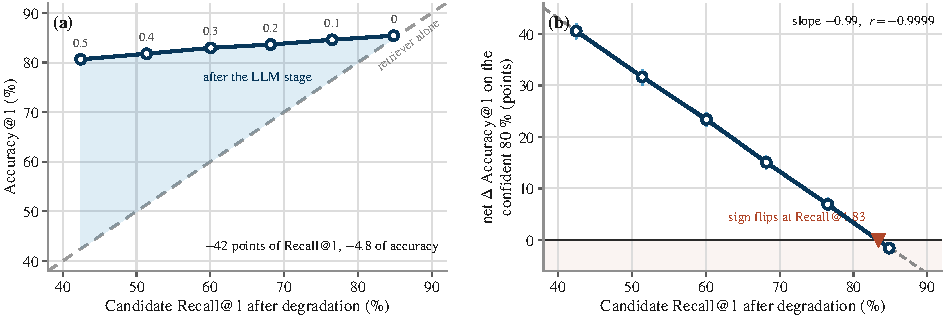
\includegraphics[width=\textwidth]{fig6_dose.pdf}
\caption{\textbf{Graded retriever degradation on a fixed candidate pool.} Starting
from BioSyn's BC5CDR candidate lists, the concept at rank 1 is swapped with a
uniformly drawn rank in $[2,10]$ for a fraction $p$ of mentions. The score vector
stays in place, so the list is still sorted, the top1$-$top2 gap distribution is
unchanged, and \rone{}@10 is $90.5$ at every level \emph{by construction}. Only which
concept sits on top changes. \textbf{(a)} The retriever loses $42.4$ points of
\rone{}; final accuracy loses $4.8$. The shaded wedge is the LLM stage's
contribution, and it grows exactly as fast as the retriever's loss.
\textbf{(b)} On the confident $80\%$ of mentions the stage's effect is a linear
function of retriever quality that crosses zero at \rone{} $\approx 83$.}
\label{fig:dose}
\end{figure*}

\subsection{A controlled dose-response}\label{sec:dose}

The relation above is observational: swapping retrievers moves the candidate pool,
the score scale and top-1 accuracy together. To manipulate one factor alone we take
BioSyn's BC5CDR candidate lists and, for a fraction $p$ of mentions, swap the concept
at rank~1 with a uniformly drawn rank in $[2,10]$, leaving the score vector in place.
The candidate set, the score distribution and the confidence signal are therefore
identical at every level --- \rone{}@10 is $90.5$ throughout --- and only the
retriever's top-1 accuracy falls, from $84.8$ at $p=0$ to $42.4$ at $p=0.5$.

Two things follow (Figure~\ref{fig:dose}). First, the stage absorbs the damage: a
$42.4$-point loss of \rone{} costs only $4.8$ points of final accuracy, so the LLM
recovers $89\%$ of what the retriever gives up, and its gain is an almost exactly
linear function of retriever quality (slope $-0.89$ points per point,
$r = -1.0000$). That is the substitution above, measured causally rather than
inferred across corpora. Second, the effect on the confident
majority is linear in the same way and \emph{changes sign}: it runs from $+40.6$
points at $p=0.5$ to $-1.6$ at $p=0$, crossing zero at \rone{} $\approx 83$
(slope $-0.99$, $r=-0.9999$). The danger zone is not a property of a particular
retriever but of retriever accuracy itself.

One thing this design deliberately does not vary is recall: degrading the ranking
leaves the gold concept in the list, whereas a genuinely weaker retriever also
retrieves it less often (BM25 reaches \rone{}@10 $79.1$ against BioSyn's $90.5$).
The controlled slope of $-0.89$ is therefore an upper bound on what swapping real
retrievers buys, and the smaller observational slope of $-0.32$ is what one should
expect when recall and ranking move together.

\section{A Mid-Confidence Danger Zone}\label{sec:f1}

\begin{figure*}[t]
\centering
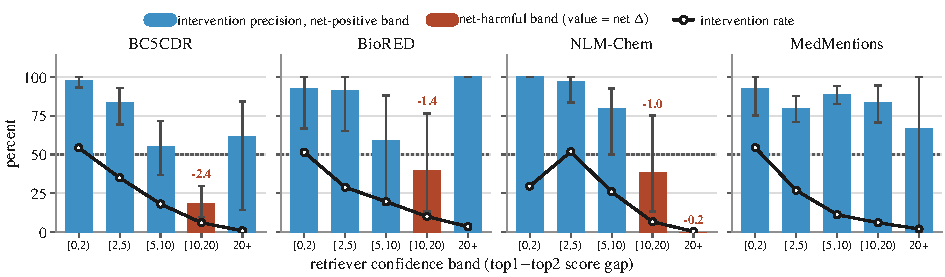
\includegraphics[width=\textwidth]{fig3_dangerzone.pdf}
\caption{\textbf{The intervention rate is calibrated; the intervention precision is
not.} Per confidence band: how often the zero-shot LLM changes the retriever's top-1
(line) and how often such a change is an improvement (bars, document-level bootstrap
95\% CI). The rate falls monotonically, but precision collapses in a mid-high band, not
at the extreme; bands where the stage is net-harmful are marked with their $\Delta$.
The pattern is absent on MedMentions, where the retriever is too weak for an override
to cost anything.}
\label{fig:danger}
\end{figure*}

\subsection{The mechanism}

The zero-shot model's intervention \emph{rate} behaves sensibly: on BC5CDR it falls
monotonically from 54.3\% of the most-uncertain mentions to 0.9\% of the most-certain
ones, and likewise on every other corpus (Figure~\ref{fig:danger}, line). It acts less
when the retriever is sure.

Its \emph{precision} does not track its rate. It is near-perfect where the retriever
is unsure (BC5CDR 98\% at gap $[0,2)$) but collapses in a mid-high band rather than at
the extreme: at gap $[10,20)$ the model still intervenes on 6.1\% of mentions and is
right only 18\% of the time (95\% CI $[10,30]$; 20 fixes against 89 breaks), turning a
stage that is strongly positive elsewhere into a net $-2.4$ points there. The retriever
is already correct on 86.5\% of those mentions, so most interventions overturn a
correct answer. The naive reading --- ``the more confident the retriever, the more
harmful the LLM'' --- is wrong: the topmost band (gap $20+$) is \emph{not} net-harmful
($+0.2$), and its precision is too noisy to interpret (rate $<1\%$, CI $[14,84]$). The
harm is localised to a middle band where the model is confident enough to act while the
retriever is already reliable.

\subsection{Where it replicates and where it does not}

The net-harmful band reproduces on BioRED ($-1.4$; precision 39\%, CI $[13,76]$),
NCBI-Disease ($-7.6$; every one of the 29 interventions in that band is a break or
lateral, 0 fixes against 19 breaks, on 249 mentions) and NLM-Chem ($-1.0$; precision 38\%,
CI $[13,75]$), but not equally robustly: under the de-duplicated protocols of
Appendix~\ref{sec:appendix-proto} the band survives on BC5CDR and NCBI-Disease and disappears on BioRED
and NLM-Chem, where it rests on a few hundred mentions. We therefore claim replication
for BC5CDR (two retrievers) and NCBI-Disease, and report BioRED and NLM-Chem as
protocol-dependent. On MedMentions, linked against the full UMLS, no band is
net-harmful under any protocol.

For NLM-Chem we can be more definite than ``protocol-dependent'', because the earlier
figure came from a 1{,}500-mention subsample. Re-running the zero-shot baseline over the
full test set puts $3{,}623$ mentions in the band --- a $7.6\times$ increase --- and the
band is still not distinguishable from zero: $\Delta = -0.33$, document-level bootstrap
CI $[-2.68, +1.69]$. Notably the interval barely narrows (it was $[-3.96,+1.44]$ on the
subsample), because NLM-Chem's $50$ full-text documents, not its mentions, are the
resampling unit and therefore the binding constraint. The absence of a band on NLM-Chem
is thus a result rather than a sample-size artefact, and no larger run on this corpus
would settle it further.
This is what the mechanism predicts: an inversion only costs accuracy when the
retriever's mid-confidence answers are usually right. On MedMentions the retriever is
weak (\rone{} 49.6--55.3\%), so even its moderately confident top-1 is often wrong and
the LLM has room to help; on the MeSH corpora the mid-confidence top-1 is mostly
right, so overriding it is expensive.

To check that this is not an artefact of our own rule-based confidence score, we repeat
the BC5CDR analysis with candidates and scores taken purely from two public retrievers.
On the weaker \emph{SapBERT} bi-encoder (\rone{} 75.9\%, the retriever used by
\citealp{ye-mitchell-2025-llm} and \citealp{lin-etal-2025-guiding}) every band is
net-positive. On the stronger \emph{BioSyn} (\rone{} 84.8\%) the danger zone reappears
with an entirely external confidence signal: precision falls to 34\% and 23\% in the
$[5,10)$ and $[10,20)$ bands, net $-2.5$ and $-1.7$ points, while the low-confidence
bands stay strongly positive ($+17.7$, $+7.2$). The effect therefore tracks retriever
strength rather than our implementation. It is an instance of what
\citet{doku-2026-confidence} call an inversion zone --- a region where higher
confidence does not mean the intervention is safer --- although we do not rely on that
work's formal apparatus for any claim here.

\paragraph{Not a surface-form artefact.}
One might suspect the score gap is a proxy for how easy the mention string is, so
that the danger zone only says the LLM should not touch exact string matches. The gap
correlates with mention--label surface similarity only moderately
($\rho = 0.38$--$0.50$), and the band structure survives stratifying on it: among the
BC5CDR mentions below surface similarity $80$ --- the hard forms, where the stage does
essentially all of its work --- $\Delta$ runs $+22.8$, $+13.1$, $+1.2$,
$\mathbf{-4.6}$, $+0.9$ across the five bands, with precision $99$, $85$, $54$,
$\mathbf{18}$, $64\%$. Above similarity $95$ the model intervenes on $0.2\%$ of
mentions, so nothing happens there either way.

\begin{figure*}[t]
\centering
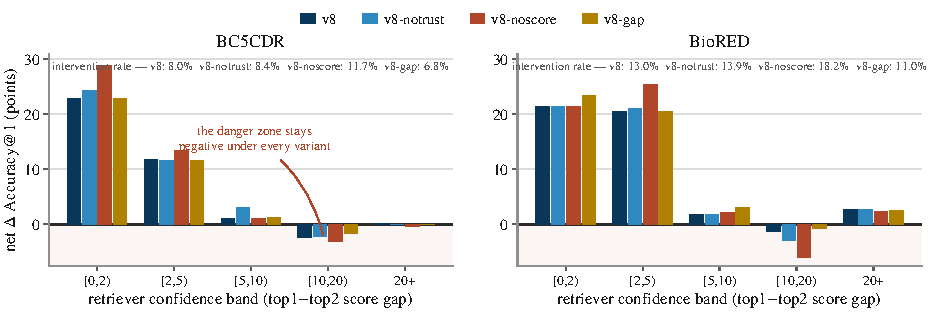
\includegraphics[width=\textwidth]{fig7_prompt.pdf}
\caption{\textbf{The danger zone survives every prompt intervention we tried.} Net
$\Delta$ \acc{} per confidence band for the prompt used throughout the paper (v8)
and three single-factor variants. v8 already tells the model to trust the ranking
\emph{and} shows it every candidate's match score. Removing the scores makes the
stage act more and decide worse; removing the verbal instruction changes almost
nothing; stating the margin as a number and telling the model how to use it halves
the net-harmful band without removing it.}
\label{fig:prompt}
\end{figure*}

\subsection{Robustness: the prompt}\label{sec:promptabl}

The obvious objection to a behavioural finding is that the prompt invited the
behaviour. It did not. The prompt used for every run in this paper already contains
the instruction \emph{``the top-ranked candidate is correct in roughly 80\% of
cases; override it only when the context gives you clear evidence''}, and it already
lists each candidate's retriever score, from which the margin is one subtraction
away. The danger zone appears anyway.

To measure what those two ingredients do, we re-run BC5CDR and BioRED with three
single-factor variants (Figure~\ref{fig:prompt}). \textbf{Removing the scores}
(v8-noscore) is clearly harmful: the intervention rate rises ($8.0 \to 11.7\%$ on
BC5CDR, $13.0 \to 18.2\%$ on BioRED), precision falls ($61 \to 56\%$,
$75 \to 63\%$), the net-harmful band deepens ($-2.4 \to -3.2$, $-1.4 \to -6.0$) and
BioRED loses $1.1$ points of accuracy ($p=0.041$). The numeric confidence signal is
load-bearing. \textbf{Removing the verbal instruction} (v8-notrust) does almost
nothing: $+0.24$ points on BC5CDR ($p=0.054$) and $-0.42$ on BioRED ($p=0.21$),
neither significant. \textbf{Stating the margin explicitly} as a number, with a rule
for how to use it (v8-gap), moves the model in the right direction --- the
intervention rate falls to $6.8\%$ and $11.0\%$, precision rises to $65\%$ and
$80\%$ --- and it halves the net-harmful band ($-2.4 \to -1.7$, $-1.4 \to -0.8$) but
does not remove it, and does not significantly change accuracy.

The reading we draw is narrow and, we think, the interesting one: the model responds
to a \emph{quantitative} confidence signal and barely at all to a verbal one, and
even when the margin is handed to it as a number together with an instruction to
defer on large margins, it still over-rides a mostly-correct retriever often enough
to lose accuracy. The inversion is not a prompt-engineering oversight.

\paragraph{Sensitivity to the evaluation protocol.}
Scoring every annotated mention occurrence over-weights frequent mention strings
\citep{tutubalina-etal-2020-fair}, which changes \emph{which} mentions dominate each
band. We therefore recompute everything under two stricter protocols --- unique
(document, mention, concept) triples, and globally unique mention--concept pairs
(Appendix~\ref{sec:appendix-proto}). The band is unchanged on BC5CDR, where on BioSyn
it in fact deepens under de-duplication ($-2.5 \to -5.0$ at gap $[5,10)$), and
unchanged on NCBI-Disease; it vanishes on BioRED and NLM-Chem, whose $[10,20)$ bands
hold only $205$ and $174$ unique pairs. The deference result of \S\ref{sec:f2} is
robust and in fact cleaner on unique pairs.

\subsection{Robustness: the disambiguator}\label{sec:models}

\begin{table}[t]
\centering\small
\setlength{\tabcolsep}{3.2pt}
\begin{tabular}{llrrrr}
\toprule
Corpus & Disambiguator & gain & band & agg. & skill \\
\midrule
BC5CDR & Qwen3-4B & \textbf{+0.9} & \textbf{--2.4} & 0.45 & 1.36 \\
 & Qwen3-8B & \textbf{+1.8} & \textbf{--1.2} & 0.46 & 2.14 \\
 & Granite-8B & \textbf{--1.5} & \textbf{--4.1} & \textbf{1.05} & 2.07 \\
\addlinespace[1pt]
BioRED & Qwen3-4B & \textbf{+4.0} & --1.4 & 0.80 & 3.13 \\
 & Qwen3-8B & \textbf{+4.6} & --1.4 & 0.71 & 2.94 \\
 & Granite-8B & +1.8 & --3.5 & \textbf{1.12} & 2.35 \\
\addlinespace[1pt]
NCBI & Qwen3-4B & +2.4 & \textbf{--7.6} & \textbf{1.12} & 0.00 \\
 & Qwen3-8B & \textbf{+6.5} & --3.2 & 0.81 & 1.60 \\
 & Granite-8B & +2.2 & \textbf{--9.2} & \textbf{1.81} & 1.45 \\
\addlinespace[1pt]
NLM-Chem & Qwen3-4B & \textbf{+5.1} & --0.3 & 0.50 & 3.94 \\
 & Qwen3-8B & \textbf{+6.9} & +0.8 & 0.45 & 6.25 \\
 & Granite-8B & \textbf{+5.2} & --0.7 & 0.90 & 3.86 \\
\bottomrule
\end{tabular}
\caption{Three disambiguators on identical mentions, candidate lists, prompt and
decoder. ``gain'' is $\Delta$ \acc{} over the whole corpus, ``band'' is $\Delta$ in gap
$[10,20)$; both are \textbf{bold} when a paired document-level bootstrap CI excludes
zero. ``agg.'' is the intervention rate in that band divided by the retriever's error
rate there, and ``skill'' is intervention precision divided by the same quantity;
neither uses \texttt{p4}, so neither restates the band column. Agg.\ above $1$ (bold)
means the model intervenes more often than the retriever is wrong and must therefore
over-ride correct predictions.}
\label{tab:models}
\end{table}

The results so far rest on one 4B model. We repeat the core measurement with
\textbf{Qwen3-8B} (same family, double the size) and \textbf{Granite-3.1-8B-Instruct}
(different family, same size as Qwen3-8B) on four corpora, holding the mentions,
candidate lists, prompt, temperature and constrained decoder fixed (Table~\ref{tab:models}).

Across the twelve model--corpus cells the net-harmful band is significantly negative in
five, indistinguishable from zero in seven, and \emph{significantly positive in none}.
It is not a property of Qwen3-4B: Granite, a different family at twice the size, shows
it more strongly than our base model does (NCBI-Disease $-9.2$, CI $[-14.1,-4.7]$;
BC5CDR $-4.1$, CI $[-5.8,-2.6]$). Nor is it a property of small models. Qwen3-8B does
attenuate it significantly relative to the 4B (BC5CDR $+1.18$, CI $[+0.23,+2.20]$;
NCBI-Disease $+4.42$, CI $[+0.79,+9.41]$), but Granite at the same parameter count is
worse than the 4B everywhere. Scale is not the variable; the model is.

One cell deserves emphasis because it is the frame of \S\ref{sec:frame} realised without
any manipulation on our part. \textbf{On BC5CDR, Granite's disambiguation stage makes
the pipeline significantly worse}: accuracy $81.3$ against a retriever at $82.7$, a net
$-1.5$ with CI $[-2.6,-0.2]$. Behind the strongest retriever in our set, a competent,
widely used 8B instruction model is a net cost.

The two right-hand columns say why, and they are the sharper version of \S\ref{sec:f1}'s
mechanism. Normalising against the retriever's error rate in the same band separates
\emph{how much} a model intervenes from \emph{how well} it chooses, and neither quantity
uses the outcome. The Qwen models modulate: on BC5CDR the aggressiveness ratio falls
$0.66 \to 0.53 \to 0.52 \to 0.45 \to 0.15$ across the five bands, so they act far less
often, relative to the opportunity, where the retriever is reliable. Granite does not:
its profile is $0.91, 0.85, 0.86, 1.05, 0.93$ --- essentially flat, and above $1$ in the
harmful band, where intervening more often than the retriever errs \emph{guarantees}
over-riding correct answers. The same holds on BioRED and NCBI-Disease. Ranked by harm,
the four worst cells in Table~\ref{tab:models} ($-9.2$, $-7.6$, $-4.1$, $-3.5$) are
exactly the four with an aggressiveness ratio above $1$.

Granite is not worse at \emph{choosing}. Its selection skill in the harmful band ($2.07$
on BC5CDR) is above the 4B's ($1.36$); both are far below the ratio needed to break even
there ($3.7$). What separates the models is not judgement but allocation --- the same
distinction fine-tuning turns out to act on (\S\ref{sec:f2}) and the same distinction a
non-generative stage turns out to obey (\S\ref{sec:ce}).

\subsection{Is a language model needed at all?}\label{sec:ce}

\begin{table}[t]
\centering\footnotesize
\setlength{\tabcolsep}{3.0pt}
\newcommand{\ci}[3]{#1$^{\,\text{\tiny #3}}_{\,\text{\tiny #2}}$}
\begin{tabular}{lrrrl}
\toprule
& \multicolumn{3}{c}{$\Delta$ \acc{} of the stage} & \\
\cmidrule(lr){2-4}
Corpus & LLM & CE$_{\text{zs}}$ & CE$_{\text{ft}}$ & CE$_{\text{ft}}-$LLM \\
\midrule
BC5CDR$^\dagger$ & +0.9 & --45.8 & +3.1 & \ci{\textbf{+2.14}}{+1.00}{+3.29} \\
BioRED & +4.0 & --47.1 & +3.6 & \ci{--0.42}{--3.36}{+2.38} \\
NCBI & +2.4 & --30.7 & +1.0 & \ci{--1.39}{--7.30}{+4.16} \\
NLM-Chem & +5.1 & --45.7 & +0.4 & \ci{\textbf{--4.67}}{--8.60}{--0.56} \\
\bottomrule
\end{tabular}
\caption{A $109$M-parameter cross-encoder on the \emph{identical} candidate lists,
against the $4$B zero-shot LLM; the retrievers are those of Table~\ref{tab:models}.
CE$_{\text{zs}}$ is MedCPT off the shelf;
CE$_{\text{ft}}$ is the same model trained on the BC5CDR training split with a listwise
objective over the same lists. The last column is the paired document-bootstrap
difference with its $95\%$ interval as sub/superscript, \textbf{bold} when it excludes
zero. $^\dagger$in-domain for CE$_{\text{ft}}$; the other three corpora are held out,
the same split structure as \S\ref{sec:f2}.}
\label{tab:ce}
\end{table}

Everything so far compares generative disambiguators with each other. The question a
practitioner asks first is different: does the stage need to be a language model? We put
a cross-encoder on the same candidate lists --- same mentions, same top-$10$, same
names, definitions and sentence --- and score it with the same code, so the document
bootstrap is exactly paired (Table~\ref{tab:ce}). We use MedCPT
\citep{jin-etal-2023-medcpt}, a $109$M-parameter biomedical re-ranker, about $1/40$ the
size of the disambiguator, in two variants: off the shelf, and trained on the BC5CDR
training split with a listwise objective over the candidate lists --- the same task the
LLM is given, and the re-ranker counterpart of \S\ref{sec:f2}'s LoRA run.

\paragraph{Off the shelf it fails, informatively.} The zero-shot cross-encoder loses
$31$ to $47$ points on every corpus, intervening on $61$--$72\%$ of mentions at an
intervention precision of $4$--$17\%$. Its selection skill is below $1$ in
\emph{all twenty} band$\times$corpus cells (range $0.00$--$0.79$): it does not merely
over-ride too often, it chooses worse than blind over-riding would. A retrieval
cross-encoder does not transfer to concept ranking without training. We report it
because it is the configuration a reader would reach for first, and because it sets the
floor the trained variant has to clear.

\paragraph{Trained, it beats the LLM in-domain.} On BC5CDR the $109$M cross-encoder adds
$+3.1$ points against the $4$B model's $+0.9$, a paired difference of $+2.14$ with a CI
that excludes zero. On the corpus you can train on, the generative stage buys nothing
that a re-ranker two orders of magnitude smaller does not buy more of. It also removes
the inversion zone: band $[10,20)$ goes from $-2.4$ under the LLM to $+1.4$, the only
positive value for that band anywhere in this paper. The danger zone is therefore not
inevitable --- it is what a stage does when its aggressiveness is not conditioned on
retriever confidence, and a stage trained on this distribution conditions correctly.

\paragraph{Out of domain the advantage is gone.} On BioRED and NCBI-Disease the
difference from the LLM is indistinguishable from zero, and on NLM-Chem the LLM is
significantly better ($-4.67$, CI $[-8.60,-0.56]$). Against the \emph{equally trained}
LLM of Table~\ref{tab:ft}, on the three corpora whose mention sets match, the gap widens
with distance from the training data: $86.5$ vs.\ $85.8$ in-domain, $85.0$ vs.\ $83.1$
on BioRED, $77.9$ vs.\ $71.1$ on NCBI-Disease. This is \S\ref{sec:f2}'s deference
result in a second model class: what training buys a re-ranking stage is bound to the
distribution it was trained on, and the LLM's residual contribution is transfer rather
than disambiguation as such.

The calibration columns say it in the mechanism's own terms. In-domain the trained
cross-encoder's aggressiveness ratio is flat at $1.01, 0.98, 0.98, 1.01, 0.45$ --- it
intervenes about as often as the retriever errs, and backs off only where the retriever
is overwhelming. On the held-out corpora the same model rises \emph{above} $1$ in the
two most confident bands ($1.27$ and $1.92$ on NCBI-Disease, $1.19$ and $1.88$ on
NLM-Chem), over-riding more often than the retriever is wrong exactly where it is most
reliable. That is Granite's profile from Table~\ref{tab:models}, produced here by a
model with no generative capacity at all. The failure mode we have been describing is
not a property of language models; it is a property of a re-ranking stage whose
allocation is not tied to the retriever's confidence.

For deployment the reading is concrete. Where the target distribution is available for
training, a $109$M re-ranker is the better purchase. Where it is not --- a new corpus, a
new entity type, a knowledge base that moves --- the LLM is the stage that survives the
shift, and that, rather than raw disambiguation skill, is what the generative stage is
being paid for.

\subsection{The consequence: a confidence gate}

\begin{table}[t]
\centering\footnotesize
\setlength{\tabcolsep}{2.6pt}
\begin{tabular}{llrrrr}
\toprule
Corpus & Retriever & full & gate & calls & gate$-$full \\
\midrule
BC5CDR & BioSyn & 85.1 & 86.3 & 18 & $+1.21_{\pm.27}$ \\
 & pipeline & 83.6 & 84.2 & 14 & $+0.55_{\pm.27}$ \\
 & SapBERT & 80.4 & 80.4 & 99 & $+0.01_{\pm.01}$ \\
BioRED & pipeline & 83.9 & 82.8 & 47 & $-1.11_{\pm.92}$ \\
NCBI & pipeline & 72.0 & 73.4 & 31 & $+1.43_{\pm1.5}$ \\
NLM-Chem & dense & 77.7 & 78.2 & 41 & $+0.54_{\pm.42}$ \\
MedMent. & SapBERT & 59.7 & 59.6 & 92 & $-0.03_{\pm.04}$ \\
\midrule
\multicolumn{6}{l}{\emph{fine-tuned control}} \\
BC5CDR & pipeline & 86.2 & 86.1 & 79 & $-0.14_{\pm.17}$ \\
\bottomrule
\end{tabular}
\caption{Confidence gate: call the LLM only when the retriever's top1$-$top2 gap is
below a threshold tuned on half the \emph{documents} and evaluated on the other half.
``full'' is the accuracy of calling the LLM on every mention, ``gate'' that of the
gated system and ``calls'' the share of mentions it sends to the LLM; all are means
over 20 random document splits, and the last column carries the standard deviation of
the difference across splits. The gate helps where the
retriever is strong enough to have produced a danger zone, is neutral where it is not,
and is harmful on BioRED. On the fine-tuned model it no longer helps, because
fine-tuning has removed the band it exploits (\S\ref{sec:f2}).}
\label{tab:gate}
\end{table}

Because the harm is confined to a predictable band, a simple policy addresses it: call
the LLM only when the retriever's gap is below a threshold, otherwise keep the
retriever's answer. To avoid tuning on the reported set we split documents in half,
choose the threshold on one half and report on the other, repeating over 20 random
splits (Table~\ref{tab:gate}).

The result is two-sided, and we state the negative half plainly. Behind the two
strongest BC5CDR retrievers the gate \emph{beats} calling the LLM everywhere:
$+1.21\pm0.27$ points at 18\% of the calls on BioSyn and $+0.55\pm0.27$ at 14\% on the
rule pipeline. Behind the weaker SapBERT retriever it is exactly neutral and selects
essentially every mention (99\% of calls), as does MedMentions (92\%) --- there is no
band to remove. On BioRED the gate is \emph{worse} than the full LLM by
$1.11\pm0.92$ points: the corpus has a net-harmful band, but it is small relative to
the gains the stage makes elsewhere, and a single scalar threshold cannot excise it
without also discarding those. The honest summary is not ``less is more'' but
``gating pays exactly where a strong retriever has created an inversion zone, and
should be validated per deployment rather than assumed''.

\section{Fine-Tuning Buys Deference, Not Competence}\label{sec:f2}

\begin{figure*}[t]
\centering
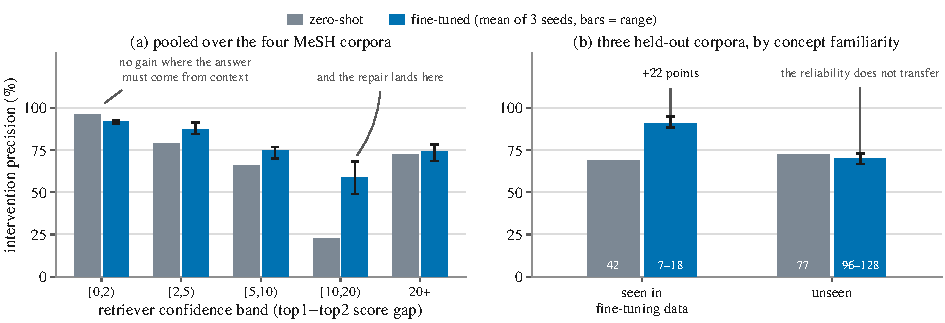
\includegraphics[width=\textwidth]{fig4_deference.pdf}
\caption{\textbf{What LoRA fine-tuning changes.} Means over three training seeds; error
bars give the range. \textbf{(a)} Intervention precision per confidence band, pooled
over the four MeSH corpora. On the truly-uncertain band the fine-tuned model is no more
precise than the zero-shot one --- slightly less so; the gains sit in the bands where
the retriever is already mostly right. \textbf{(b)} Intervention precision on three
corpora the model never trained on, split by whether the gold concept occurs in the
fine-tuning data. The reliability fine-tuning buys is realised on seen concepts and is
absent on unseen ones, where precision in fact declines; numbers inside the bars are
breaks.}
\label{fig:deference}
\end{figure*}

\begin{table}[t]
\centering\small
\setlength{\tabcolsep}{3.2pt}
\newcommand{\rng}[3]{#1$^{\,\text{\tiny #3}}_{\,\text{\tiny #2}}$}
\begin{tabular}{lrrlrlr}
\toprule
& & \multicolumn{2}{c}{P4} & \multicolumn{2}{c}{prec.} & \\
\cmidrule(lr){3-4}\cmidrule(lr){5-6}
Corpus & R@1 & zs & ft & zs & ft & $p$ \\
\midrule
BC5CDR$^\dagger$ & 82.7 & 83.7 & \rng{86.5}{86.0}{86.8} & 61 & \rng{82}{77}{87} & $<$.001 \\
BioRED & 79.5 & 83.6 & \rng{85.0}{84.8}{85.1} & 75 & \rng{77}{75}{80} & $\leq$.028 \\
NCBI & 70.1 & 72.5 & \rng{77.9}{76.9}{79.4} & 58 & \rng{74}{70}{82} & $<$.001 \\
NLM-Chem & 72.3 & 78.0 & \rng{79.4}{78.6}{79.9} & 80 & \rng{76}{73}{78} & .005--.43 \\
\bottomrule
\end{tabular}
\caption{Zero-shot (zs) vs.\ LoRA fine-tuned (ft) disambiguator on the identical
mentions and identical candidate lists; ``prec.'' is overall intervention precision.
Fine-tuned entries are the mean over \textbf{three training seeds}, with the observed
range over seeds set as the sub/superscript, and $p$ is the largest (worst) exact McNemar test over those three seeds.
$^\dagger$in-domain: the model was fine-tuned on the BC5CDR training split; the other
three corpora are held out. Accuracy improves on every corpus and every seed, but on
NLM-Chem the improvement is not significant on one of the three ($p=.43$), and overall
intervention precision improves only where it was low to begin with --- on BioRED and
NLM-Chem, where the zero-shot model was already precise, fine-tuning does not add to it
and on NLM-Chem slightly reduces it.}
\label{tab:ft}
\end{table}

Fine-tuning raises accuracy on all four corpora (Table~\ref{tab:ft}). The question is
\emph{what} it improves. Every number in this section is the mean over three training
seeds, which differ only in weight initialisation and data order; the ranges matter,
because a single run overstates two of the effects below.

\paragraph{Competence does not improve; allocation does.}
Read by confidence band (Figure~\ref{fig:deference}a), fine-tuning does not make the
model a better disambiguator where disambiguation is hard. On the truly-uncertain band
$[0,2)$, where the answer has to come from context, pooled intervention precision does
not rise --- it falls slightly, $96.1\% \to 91.6\%$ (range $90.6$--$92.5$). The model
acts \emph{more} often there and nets more repairs (fixes $149 \to 228$), but its
accuracy per intervention is no better than before, and breaks appear where the
zero-shot model had almost none ($6 \to 21$).

What changes is where the interventions go. Fine-tuning does not make the model quieter:
on BC5CDR the overall intervention rate \emph{rises}, $8.0\% \to 10.0\%$. It redirects
them. In the band $[10,20)$, where the retriever is already right on $86.5\%$ of
mentions, precision goes from $18\%$ to $62\%$ (range $50$--$74$) and the net effect
from $\Delta = -2.4$ to $\Delta = +0.7$ (range $-0.0$ to $+1.3$); in the two bands where
the retriever is usually wrong the model intervenes markedly more. Fine-tuning buys the
gate of \S\ref{sec:f1}, learned internally, and consistently the external gate no longer
beats the full LLM on the fine-tuned model (Table~\ref{tab:gate}, last row).

The band repair is not universal, and here the seeds correct a single-run result. It is
strong on BC5CDR and on NLM-Chem ($38\% \to 72\%$, range $67$--$76$; $\Delta$ $-1.0 \to
+2.9$), partial and still centred on zero on NCBI-Disease ($0\% \to 50\%$, range
$36$--$70$; $\Delta$ $-7.6 \to -0.4$, range $-1.6$ to $+1.6$), and \emph{absent} on
BioRED, where precision in that band stays at $39\%$ (range $38$--$41$) and the band
remains net-harmful ($-1.4 \to -1.2$). A single fine-tuning run had suggested $69\%$ on
BioRED; none of the three seeds reproduces it. BioRED is the same corpus on which the
danger zone did not survive de-duplication (\S\ref{sec:f1}) and on which the confidence
gate loses (Table~\ref{tab:gate}) --- three independent checks pointing the same way.

\paragraph{The restraint is bound to the training distribution.}
Whether this restraint \emph{transfers} depends on whether the concept was in the
fine-tuning data. Pooling the three corpora the model never trained on (BioRED,
NCBI-Disease, NLM-Chem; 4{,}024 mentions), fine-tuning raises intervention precision on
\emph{seen} concepts from $68.7\%$ to $90.5\%$ (range $88.2$--$94.9$ over the three
seeds), while on \emph{unseen} concepts it does not improve at all: $72.2\% \to 69.8\%$
(range $66.7$--$73.0$). The two seed ranges do not overlap, and the direction differs:
breaks on seen concepts fall from $42$ to $7$--$17$, while breaks on unseen concepts
\emph{rise} from $77$ to $96$--$128$.

The band breakdown localises it. On seen concepts the gain is confined to exactly the
bands where the danger zone lived --- $+23$ points at gap $[5,10)$ and $+50$ at
$[10,20)$, with $[0,2)$, $[2,5)$ and $20+$ unchanged. On unseen concepts no band gains:
$-11$, $+7$, $-4$, $+5$, $-27$ across the five. Unlike the danger zone, this contrast
does not depend on the evaluation protocol; on globally unique mention--concept pairs it
is sharper still, $65.9\% \to 87.5\%$ (range $86.2$--$89.5$) on seen concepts against
$70.6\% \to 64.2\%$ (range $60.9$--$66.7$) on unseen ones, where the unseen side moves
clearly \emph{down}.

We therefore make the claim the data support: fine-tuning installs a
confidence-dependent restraint, and that restraint is a property of the concepts it was
trained on rather than a policy it applies to new ones. Accuracy still improves
out-of-domain (Table~\ref{tab:ft}), so the model is not worse overall on novel concepts
--- but it buys that improvement by intervening more, not by choosing better, and the
near-perfect reliability it appears to acquire does not come with it.

\section{An Anatomy of the Interventions}\label{sec:f3}

The zero-shot model changes the retriever's top-1 on $8.0\%$ of BC5CDR mentions (771
of $9{,}661$): $33\%$ fixes, $21\%$ breaks, $46\%$ lateral. Splitting the lateral
moves matters, because only $14.5$ of those $46$ points occur when the gold concept
was in the candidate list at all --- genuine confusion --- while the remaining $31.5$
are lateral by construction, the gold having never been retrieved. The
genuine-confusion rate is therefore about $15\%$ of all changes, not $46\%$
(Appendix~\ref{sec:appendix-churn}). Two quantities bound what the stage can do: of
the retriever's errors whose gold \emph{is} in the candidate list it recovers $24\%$
(MedMentions) to $66\%$ (BC5CDR/BioSyn), $30\%$ on the BC5CDR rule pipeline; and on
that run $809$ of the $1{,}667$ retriever errors have no gold concept in the list, so
no disambiguator could fix them. Averaged over the three fine-tuning seeds the picture
sharpens the account of \S\ref{sec:f2}: the model makes \emph{more} changes ($771 \to
970$), raises fixes to $48\%$ (range $44$--$50$) and halves breaks to $10\%$ (range
$8$--$13$), while genuine confusion barely moves ($14.5\% \to 9.9\%$, range
$9.7$--$10.2$) and the share of changes that were lost before the LLM saw them is
unchanged at $32\%$. Recovery on the repairable errors rises from $29\%$ to $54\%$
(range $53$--$56$) --- almost entirely by attempting more of them, not by confusing
fewer. The stage is best described as
over-eager where there is nothing to gain and under-powered where it matters. The
pattern is not driven by entity type: on BC5CDR the stage adds $+1.0$ points on the
$5{,}351$ chemical mentions and $+0.9$ on the $4{,}310$ disease mentions.

\section{Discussion}

One account ties the results together. The LLM disambiguation stage is not a general
semantic reasoner applied uniformly to a candidate list; it is a
retriever-dependent, mechanically bounded correction, valuable exactly where the
retriever is uncertain and idle-to-harmful on the confident majority. Fine-tuning does
not lift its ceiling on the hard cases; it teaches the model \emph{when} to defer, and
that deference is calibrated to the concepts it was trained on.

Three consequences follow for practice. Reported gains from an LLM disambiguation
stage are statements about a retriever--LLM pair and should be reproduced against the
retriever the authors used before being attributed to the model. Behind a strong
retriever the stage should be gated or cascaded, but the gate must be validated on
the target corpus --- it helped on three of our seven configurations, was neutral on
two and hurt on one. And a fine-tuned disambiguator should be expected to be reliable
on familiar concepts and merely adequate on novel ones, which is precisely the regime
biomedical deployment cares about.

\section*{Limitations}

\paragraph{The re-ranker baseline is one architecture and one recipe.} The
cross-encoder of \S\ref{sec:ce} is MedCPT initialised, trained with a listwise objective
on BC5CDR only, one seed. That matches \S\ref{sec:f2}'s LoRA setup by design, so
``held out'' means the same thing on both sides, but it leaves the obvious stronger
baseline untested: a re-ranker trained on all four corpora, or a bi-encoder--cross-encoder
architecture built for entity linking rather than passage retrieval, might transfer
where ours does not. Our transfer claim is therefore about \emph{this} re-ranker
against \emph{this} LLM under a matched training budget, not about the two model
classes in general.

\paragraph{Fine-tuning is one recipe.} The deference result uses LoRA SFT on the gold
answer, over three seeds. It does not tell us what a different objective would buy. The
distinction the paper keeps arriving at --- that the failure is allocation rather than
judgement --- suggests a reward that scores the \emph{decision} (repair, break, abstain)
rather than the answer, which supervised fine-tuning on gold labels cannot express. We
have not tested that.

\paragraph{The degradation varies ranking, not recall.} The dose-response of
\S\ref{sec:dose} holds \rone{}@10 fixed by construction, so it measures the stage's
ability to repair a mis-\emph{ranked} candidate list, not its value behind a
retriever that fails to retrieve the gold concept at all. Real retrievers differ on
both axes, which is why the controlled slope ($-0.89$) exceeds the observational one
($-0.32$). A second manipulation that removes candidates rather than reordering them
would complete the picture; we have not run it.

\paragraph{The seen/unseen split is confounded with frequency.} Concepts present in the
BC5CDR training data are also the more frequent ones, so part of the seen-concept
improvement in \S\ref{sec:f2} may reflect frequency rather than exposure. A clean
isolation stratifies within frequency bands; we have not run it.

\paragraph{Evaluation protocol.} Following BioLinkerAI we score every annotated
mention occurrence, which inflates absolute accuracies relative to de-duplicated
protocols \citep{tutubalina-etal-2020-fair} and makes our absolute numbers not
directly comparable to published leaderboards. Appendix~\ref{sec:appendix-proto} repeats the analysis under two stricter
protocols and names the two claims that do not survive them.
Separately, the BM25 run covers $9{,}391$ of the $9{,}661$ BC5CDR mentions; where the
four BC5CDR retrievers are compared directly (Figure~\ref{fig:value}a) we restrict to
the shared subset.

\paragraph{Confidence signal.} Our confidence signal is a top1$-$top2 score gap, which
is neither calibrated nor comparable across retrievers; we handle this by binning
within each run, but a calibrated retriever confidence would be a stronger instrument
and might move the location of the danger zone.

\paragraph{Scope.} We evaluate linking given gold mentions, on English abstracts and
one full-text corpus, against MeSH and UMLS. Nothing here speaks to mention detection,
to other knowledge bases, or to languages other than English.

\section*{Acknowledgments}

Anonymised for review.

\bibliography{custom}

\appendix

\section{Evaluation protocols}
\label{sec:appendix-proto}

\begin{table}[t]
\centering\footnotesize
\setlength{\tabcolsep}{3pt}
\begin{tabular}{llrrr}
\toprule
& & \multicolumn{3}{c}{net $\Delta$ (n)} \\
\cmidrule(lr){3-5}
Run & Band & occ. & doc. & uniq. \\
\midrule
BC5CDR pipeline & $[10,20)$ & $-2.4$ & $-2.2$ & $-1.5$ \\
BC5CDR BioSyn & $[5,10)$ & $-2.5$ & $-3.9$ & $-5.0$ \\
BC5CDR BioSyn & $[10,20)$ & $-1.7$ & $-1.4$ & $-1.5$ \\
NCBI & $[10,20)$ & $-7.6$ & $-5.3$ & $-6.2$ \\
\addlinespace[2pt]
BioRED & $[10,20)$ & $-1.4$ & $+0.8$ & $+1.0$ \\
NLM-Chem & $[10,20)$ & $-1.0$ & $\pm0.0$ & $\pm0.0$ \\
\bottomrule
\end{tabular}
\caption{The net-harmful band under three evaluation protocols: every annotated
mention occurrence (occ., the BioLinkerAI protocol used throughout the paper), unique
(document, mention, concept) triples (doc.), and globally unique mention--concept pairs
(uniq.). The band is protocol-independent on BC5CDR and NCBI-Disease and
protocol-dependent on BioRED and NLM-Chem.}
\label{tab:proto}
\end{table}

\section{Anatomy of the interventions}
\label{sec:appendix-churn}

\begin{figure}[h]
\centering
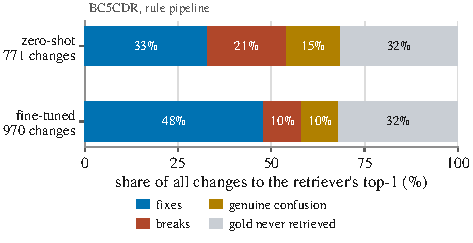
\includegraphics[width=\columnwidth]{fig5_churn.pdf}
\caption{Every change the LLM makes to the retriever's top-1, decomposed. Lateral
moves are split by whether the gold concept was in the candidate list at all: where it
was not, any change is lateral by construction and is not evidence of confusion.}
\label{fig:churn}
\end{figure}

\section{Per-band numbers}
\label{sec:appendix}

Table~\ref{tab:bands} gives the full band breakdown for the BC5CDR rule pipeline that
Figure~\ref{fig:danger} summarises. Equivalent tables for the remaining thirteen runs,
all prediction dumps, and the analysis and figure scripts are released with the paper.

\begin{table}[h]
\centering\small
\setlength{\tabcolsep}{3.4pt}
\begin{tabular}{lrrrrr}
\toprule
Band & \multicolumn{1}{c}{$n$} & rate & prec. & 95\% CI & $\Delta$ \\
\midrule
$[0,2)$    & 337   & 54.3 & 98 & [93,100] & $+22.8$ \\
$[2,5)$    & 543   & 35.0 & 83 & [69,93]  & $+11.8$ \\
$[5,10)$   & 988   & 18.1 & 55 & [37,72]  & $+1.0$ \\
$[10,20)$  & 2{,}881 & 6.1 & 18 & [10,30]  & $-2.4$ \\
$20+$      & 4{,}912 & 0.9 & 62 & [14,84]  & $+0.2$ \\
\bottomrule
\end{tabular}
\caption{BC5CDR, rule pipeline, zero-shot Qwen3-4B. Rate and precision in percent,
$\Delta$ in \acc{} points. The $20+$ band's precision rests on 34 interventions and
should not be read as a recovery.}
\label{tab:bands}
\end{table}

\end{document}
